\documentclass[12pt]{article}

\usepackage{geometry}
\geometry{a4paper} 
\usepackage{fullpage}

\usepackage{amssymb,rotating,natbib,graphicx,fancyvrb} 

\usepackage[parfill]{parskip} 
\usepackage[utf8]{inputenc}

%% double spacing
\usepackage{setspace}
\doublespacing

% line numbers
\usepackage{lineno}
\linenumbers
\renewcommand\linenumberfont{\normalfont\small}

% remove page numbers
%\pagenumbering{gobble}


%% new custom commands for code formatting
\newcommand{\code}[1]{\texttt{#1}}
\newcommand{\class}[1]{`\code{#1}'}
%\newcommand{\fct}[1]{#1}
\newcommand{\fct}[1]{\texttt{#1()}}
\newcommand{\pkg}[1]{{\fontseries{b}\selectfont #1}}
\let\proglang=\textsf


\begin{document}

\DefineVerbatimEnvironment{Code}{Verbatim}{}
\DefineVerbatimEnvironment{CodeInput}{Verbatim}{fontshape=sl}
\DefineVerbatimEnvironment{CodeOutput}{Verbatim}{}
\newenvironment{CodeChunk}{}{}

\raggedright


\textbf{Reproducible, flexible and high throughput data extraction from primary literature: The \pkg{metaDigitise} \proglang{R} package}

Joel L. Pick$^{1,*}$, Shinichi Nakagawa$^1$, Daniel W.A. Noble$^1$

$^1$
  Ecology and Evolution Research Centre, School of Biological, Earth and Environmental Sciences,  University of New South Wales, Kensington, NSW 2052, Sydney, AUSTRALIA

 $^*$Corresponding Author: joel.l.pick@gmail.com\\


\clearpage
\section*{Abstract}
\begin{enumerate} 
\item Research synthesis, such as meta-analysis requires the extraction of effect sizes from primary literature. Such effect sizes are calculated from summary statistics. However, exact values of such statistics are commonly hidden in figures. 

\item Extracting summary statistics from figures can be a slow process that is not easily reproducible. Additionally, current software lacks an ability to incorporate important meta-data (e.g., sample sizes, treatment / variable names) about experiments and is not integrated with other software to streamline analysis pipelines.

\item Here we present the R package \pkg{metaDigitise} which extracts descriptive statistics such as means, standard deviations and correlations from the four plot types: 1) mean/error plots (e.g. bar graphs with standard errors), 2) box plots, 3) scatter plots and 4) histograms. \pkg{metaDigitise} is user-friendly and easy to learn as it interactively guides the user through the data extraction process. Notably, it enables large-scale extraction by automatically loading image files, letting the user stop processing, edit and add to the resulting data fame at any point. 

\item Digitised data can be easily re-plotted and checked, facilitating reproducible data extraction from plots with little inter-observer bias. We hope that by making the process of figure extraction more flexible and easy to conduct it will improve the transparency and quality of meta-analyses in the future.
\end{enumerate}

\vskip10pt
 \textbf{Keywords:} meta-analysis, comparative analysis, data extraction, \proglang{R}, reproducibility, figures, images, summary statistics




%%%---------------------------------
%%%---------------------------------
%%%---------------------------------
\clearpage



\section{Introduction}

In many different contexts, researchers make use of data presented in primary literature. Most notably, this includes meta-analysis, which is becoming increasingly common in many research fields. Meta-analysis uses effect size estimates and their sampling variance, taken from many studies, to understand whether particular effects are common across studies and to explain variation among these effects \citep{Glass1976,Koricheva2013,Naka2017}. Meta-analysis relies on descriptive statistics (e.g. means, standard deviations (SD), sample sizes, correlation coefficients) extracted from primary literature that have been reported in the text or tables of research papers. Descriptive statistics are also, however, frequently presented in figures and so need to be manually extracted using digitising programs. While inferential statistics (e.g., \textit{t}- and \textit{F}-statistics) are often presented along side descriptive statistics, and can be used to derive effect sizes, descriptive statistics are much more appropriate to use because sources of non-independence in experimental designs can be dealt with more easily \citep{Noble2017}. 

Although there are several tools that data extraction from figures (e.g. \proglang{DataThief} \citep{DataThief}, \proglang{GraphClick} \citep{GraphClick}, \proglang{WebPlotDigitizer} \citep{WebPlotDigitizer}), these tools do not cater to needs of meta-analysis for three main reasons. First, they typically only provide the user with calibrated \textit{x,y} coordinates from imported figures, and do not differentiate between common plot types that are used to present data. Consequently a large amount of downstream data manipulation is required, that is different across plots types. For example, data are frequently presented in mean/error plots (Figure \ref{fig:all_extract}A), from which the user wants a mean and SD for each group presented. From \textit{x,y} coordinates, users must manually discern between mean and error coordinates and assign points to groups. Error then needs to be calculated as the deviation from the mean, and then transformed to SD, according to the type of error presented. Second, digitising programs do not allow the integration of metadata at the time of data extraction, such as experimental group or variable names, and sample sizes. This makes the downstream calculations laborious, as information has to be added later using different software. Finally, existing programs do not import sets of images for the user to systematically work through. Instead they require the user to manually import images one by one, and export data into individual files, that need to be imported and edited using different software. 

Data extraction from figures is therefore an incredibly time-consuming process as existing software does not provide an optimized research pipeline to facilitate data extraction and editing. Furthermore, although meta-analysis is an important tool in consolidating the data from multiple studies, many of the processes involved in data extraction are opaque and difficult to reproduce, making extending studies problematic. Having a tool that facilitates reproducibility in meta-analyses will increase transparency and aid in resolving the reproducibility crises seen in many fields \citep{peng_reproducible_2006, peng_reproducible_2011, Parker2016}.

Here, we present an interactive \proglang{R} package, \pkg{metaDigitise} (available at https://github.com/daniel1noble/metaDigitise), which is designed for large scale, reproducible data extraction from figures, specifically catering to the the needs of meta-analysts. To this end, we provide tools to extract data from common plot types (mean/error plots, box plots, scatter plots and histograms, see Figure \ref{fig:all_extract}). \pkg{metaDigitise} operates within the \proglang{R} environment making data extraction, analysis and export more streamlined. The necessary calculations are carried out on calibrated data immediately after extraction so that comparable summary statistics can be obtained quickly. Summary data from multiple figures is returned into a single data frame which can be can easily exported or use in downstream analysis within \proglang{R}. Completed digitisations are automatically saved for each figure, meaning users can redraw their digitisations on figures, make corrections and access calibration and proceeded data. This makes sharing figure digitisation and reproducing the work of others simple and easy, and allows meta-analyses to be updated more efficiently.


%% 612 words

%%%---------------------------------
%%%---------------------------------
%%%---------------------------------

\section{Directory Structure and Reproducibility}
The \pkg{metaDigitise} package was created with the idea that users would have multiple images to extract from and therefore operates in the same way whether the user has one or multiple images. There is one main function, \fct{metaDigitise}, which interactively takes the user through the process of extracting data from figures. \fct{metaDigitise} works on a directory containing images of figures copied from primary literature, in .png, .jpg, .tiff, .pdf format, specified to \fct{metaDigitise} through the \code{dir} argument. The user should think carefully about their directory structure early on in their project. Although different directory structures may be used, we would recommend having all files for one project in a single directory with an informative and unambiguous naming scheme for images to help identify the paper and figure that data come from (e.g. paper\_figure\_trait.png).

\fct{metaDigitise} recognizes all the images in a directory and automatically imports them one by one, allowing the user to extract the relevant information about a figure as they go. Having all figures in one directory therefore expedites digitisation by preventing users from having to constantly change directories and / or open new images. The data from each completed image is automatically saved as a \code{metaDigitise} object in a separate .RDS file to a \code{caldat} directory that is created within the parent directory when first executing \fct{metaDigitise}. These files enable re-plotting and editing of images at a later point (see below). When run, \fct{metaDigitise} also identifies the images within a directory that have been previously digitised and only imports new images to process. The data of all images is then automatically integrated into the final output. This means that all figures do not need to be extracted at one time and new figures can be added to the directory as the project develops.

This directory structure allows the complete digitisation process to be reproduced at a later stage, shared with collaborators and presented as supplementary materials for a publication. As long as all the images and the caldat directory are still in one directory, \fct{metaDigitise} will be able to reproduce all figure extractions, regardless of the computer it is run on. For an analysis to be updated, new figures can simply be added to the directory and \fct{metaDigitise} run to incorporate the new data. 

%% 365 words
%%%---------------------------------
%%%---------------------------------
%%%---------------------------------


\section{Image Processing}
Running \fct{metaDigitise} presents the user with three options; `Process new images', `Import existing data' or `Edit existing data'. Selecting `Process New Images' starts the digitisation process on images within the directory that have not preciously been digitised; the other functions are discussed below.

For all plot types, \fct{metaDigitise} requires the user to calibrate the axes in the figure, by clicking on two known points on the axis in question, and entering the value of those points (Figure \ref{fig:all_extract}). \fct{metaDigitise} then calculates the value of any clicked points in terms of the figure axes. This is based on the calibration used in the \pkg{digitize} R package \citep{Poisot2011}. For mean/error and box plots, only the y-axis is calibrated (Figure \ref{fig:all_extract}A,B), assuming the x-axis is redundant. For scatter plots and histograms both axes are calibrated (Figure \ref{fig:all_extract}C,D).

As figures may have been copied from older, scanned publications, they may not be perfectly orientated. This makes calibration of the points in the figure problematic. \fct{metaDigitise} allows users to rotate the image (Figure \ref{fig:rotate}A,B). Furthermore, mean/error plots, box plots and histograms, may be presented with horizontal bars. \fct{metaDigitise} assumes that bars are vertical, but allows the user to flip the image to make the bars are vertical (Figure \ref{fig:rotate}C,D).

\pkg{metaDigitise} recognises four main types of plot; Mean/error plots, box plots, scatter plots and histograms (\ref{fig:all_extract}). All plot types can be extracted in a single call of \fct{metaDigitise} and integrated into one output. Alternatively, users can process different plot types separately, using separate directories. All four plot types are extracted slightly differently (outlined below). Upon completing all images, or quitting, either summarised or calibrated data is returned (specified by the user through the \code{summary} argument). Summarised data consists of a mean, SD and sample size, for each identified group within the plot (should multiple groups exist). In the case of scatter plots, the correlation coefficient between x and y variables within each identified group is also returned. Calibrated data consists of a list with slots for each of the four figure types, containing the calibrated points that the user has clicked. This may be particularly useful in the case of scatter plots. 

\subsection{Mean/Error and Box Plots} 
\fct{metaDigitise} handles mean/error and box plots in a very similar way. For each mean/box, the user is enters group names and sample sizes. If the user does not enter a sample size at the time of data extraction (if, for example, the information is not readily available) a SD is not calculated. Sample sizes can, however, be entered at a later time (see below). For mean/error plots, the user clicks on an error bar and the mean. Error bars above or below the mean can be clicked, as sometimes one is clearer than the other. \fct{metaDigitise} assumes that the error bars are symmetrical. Points are displayed where the user has clicked, with the error in a different colour to the mean (Figure \ref{fig:all_extract}A). The user also enters the type of error used in the figure: SD, standard error (SE) or 95\% confidence intervals (CI95). For box plots, the user clicks on the maximum, upper quartile, median, lower quartile and minimum. For both plot types, the user can add, edit or remove groups. Three functions, \fct{error\_to\_sd}, \fct{rqm\_to\_mean} and \fct{rqm\_to\_sd}, that convert different error types to SD, box plot data to mean and box plot data SD, respectively, are also available in the package (see supplements for further details of these conversions).

\subsection{Scatter plots}
Users can extract points from multiple groups from scatter plots. Different groups are plotted in different colours and shapes to enable them to be distinguished, with a legend at the bottom of the figure (Figure \ref{fig:all_extract}C). Mean, SD and sample size are calculated from the clicked points, for each group. Data points may overlap with each other making it impossible to know whether points have been missed. This may result in the sample size of digitised groups conflicting with what is reported in the paper. For example, in Figure \ref{fig:all_extract}C only 49 points have been clicked when the sample size is known to be 50. Hence, \pkg{metaDigitise} also provides the user with the option to input known sample sizes directly. Nonetheless, it is important to recognise the impact that overlapping points can have on summary statistics, and in particular on sampling variance.

\subsection{Histograms}
The user clicks on the top corners of each bar, which are drawn in alternating colours (Figure \ref{fig:all_extract}D). Bars are numbered to allow the the user to edit them. As with scatter plots, if the sample size from the extracted data does not match a known sample size, the user can enter an alternate sample size. The calculation of mean, SD and sample size from this data is shown in the supplements.


%% 770 words

%%%---------------------------------
%%%---------------------------------
%%%---------------------------------

\section{Importing and Editing Previously Digitised data}
\pkg{metaDigitise} is also able to re-import, edit and re-plot previously digitised figures. When running \fct{metaDigitise}, the user can choose to `Import existing data', which returns previously digitised data, from sinlge or all figures. Alternately, the \fct{getExtracted} function returns the data of previous digitisations, but without user interaction, allowing easier integration into larger scripts. `Edit existing data' allows the user to re-plot or edit information or digitisations that have previously be done.

\subsection{Adding Sample Sizes to Previous Digitisations}
In many cases sample sizes may not be readily available when digitising figures. This information does not need to be added a the time of digitisation. To expedite finding and adding these sample sizes at a later point, \fct{metaDigitise} has a specific edit option that allows users to enter previously omitted sample sizes. This first identifies missing sample sizes in the digitised output, re-plots the relevant figures and prompts the user to enter the sample sizes for the relevant groups in the figure, one by one. 


%% 171 words


%%%---------------------------------
%%%---------------------------------
%%%---------------------------------

\section{Software Validation}
In order to evaluate the consistency of digitisation with \pkg{metaDigitise} between users, we got 14 people to digitise the same set of 14 figures created from a simulated dataset (see supplements). We found no evidence for any inter-observer variability in digitisations for the mean (ICC = 0, 95\% CI = 0 to 0.029, \textit{p} = 1), SD (ICC = 0, 95\% CI = 0 to 0.033, \textit{p} = 0.5) or correlation coefficient (ICC = 0.053, 95\% CI = 0 to 0.296, \textit{p} = 0.377). There was little bias between digitised and true values, on average 1.63\% (mean = 0.02\%, SD = 4.9\%, \textit{r} = -0.03\%) and there were small absolute differences between digitised and true values, on average 2.18\% (mean = 0.40\%, SD = 5.81\%, \textit{r} = 0.33\%) across all three summary statistics. SD estimates from digitisations are clearly most error prone. The mean absolute differences for each plot type clearly show that this effect is driven by extraction from box plots and histograms (\% difference; box plot: 15.805, histogram: 5.210, mean/error: 1.500, scatter plot: 0.433). SD estimation from box plot summary statistics is known to be more error prone, especially at small sample sizes \citep{Wan2014}. 

We also used simulated data to test the accuracy of digitisations with respect to known values (see supplements). \pkg{metaDigitise} was extremely accurate at matching clicked points to their true values essentially being perfectly correlated with the true simulated data for both the \textit{x}-variable (Pearson's correlation; \textit{r} > 0.999, \textit{t} = 2137.4, \textit{df} = 78, $p < 0.001$) and \textit{y}-variable (\textit{r} > 0.999, \textit{t} = 1897.8, \textit{df} = 78, $p < 0.001$) in scatterplots.


%% 263 words


%%%---------------------------------
%%%---------------------------------
%%%---------------------------------


\section{Limitations}

Although \pkg{metaDigitise} is very flexible and provides functionality not seen in any other package, there are some functions that it does not perform (see Table S1). Notably \pkg{metaDigitise} lacks automated point detection. However, from our experience, manual digitising is more reliable and often equally as fast. Given the variation in image quality, calibration for automatic point detection needs to be done for each figure individually. Additionally, auto-detection often misses points which then need to be manually added. Based on tests of \pkg{metaDigitise} (see above), figures can be extracted in around 1-2 minutes, including the entry of metadata. As a result, we do not believe that current automated point detection techniques provide substantial benefits in terms of time or accuracy.

\pkg{metaDigitise} also (currently) lacks the ability to zoom in on figures. Zooming may enable users to gain greater accuracy when clicking on points. However, from our own experience (see results above), with a reasonably sized screen accuracy is already high, and so relatively little gain is to be had from zooming in on points.

In contrast to some other packages \pkg{metaDigitise} does not extract lines from figures. Line extraction is not particularly useful for most meta-analyses, although we recognise that it may be useful in other fields. Should a user like to extract lines with \pkg{metaDigitise}, we would recommend extracting data as a scatter plot, and clicking along the line in question. A model can then be fitted to these points (accessed by choosing to return calibrated rather than summary data) to estimate the parameters needed.

%% 249 words


%%%---------------------------------
%%%---------------------------------
%%%---------------------------------


\section{Conclusions}
Increasing the reproducibility of figure extraction for meta-analysis and making this laborious process more streamlined, flexible and integrated with existing statistical software will go a long way in facilitating the production of high quality meta-analytic studies that can be updated in the future. We believe that \pkg{metaDigitise} will improve this research synthesis pipeline, and will hopefully become an integral package that can be added to the meta-analysts toolkit.

% 68
\section*{Acknowledgments}
We thank the I-DEEL group and colleagues at UNSW for for testing, providing feedback and digitising including: Rose O'Dea, Fonti Kar, Malgorzata Lagisz, Julia Riley, Diego Barneche, Erin Macartney, Ivan Beltran, Gihan Samarasinghe, Dax Kellie, Jonathan Noble, Yian Noble and Alison Pick. J.L.P. was supported by a Swiss National Science Foundation Early Mobility grant (P2ZHP3\_164962), D.W.A.N. was supported by an Australian Research Council Discovery Early Career Research Award (DE150101774) and UNSW Vice Chancellors Fellowship and S.N. an Australian Research Council Future Fellowship (FT130100268). 

% 153
\section*{Author Contributions}
J.L.P. and D.W.A.N. conceived the study and J.L.P., S.N. and D.W.A.N. developed the idea. J.L.P. and D.W.A.N. developed the R-package. J.L.P. and D.W.A.N. wrote the first draft of the paper and J.L.P., S.N. and D.W.A.N. contributed substantially to subsequent revisions of the manuscript and gave final approval for publication.

% 51
\bibliographystyle{FuncEcol.bst}
\bibliography{metaDigitise}


\clearpage
\section*{Figures}

\begin{figure}[!h]
\centering 
 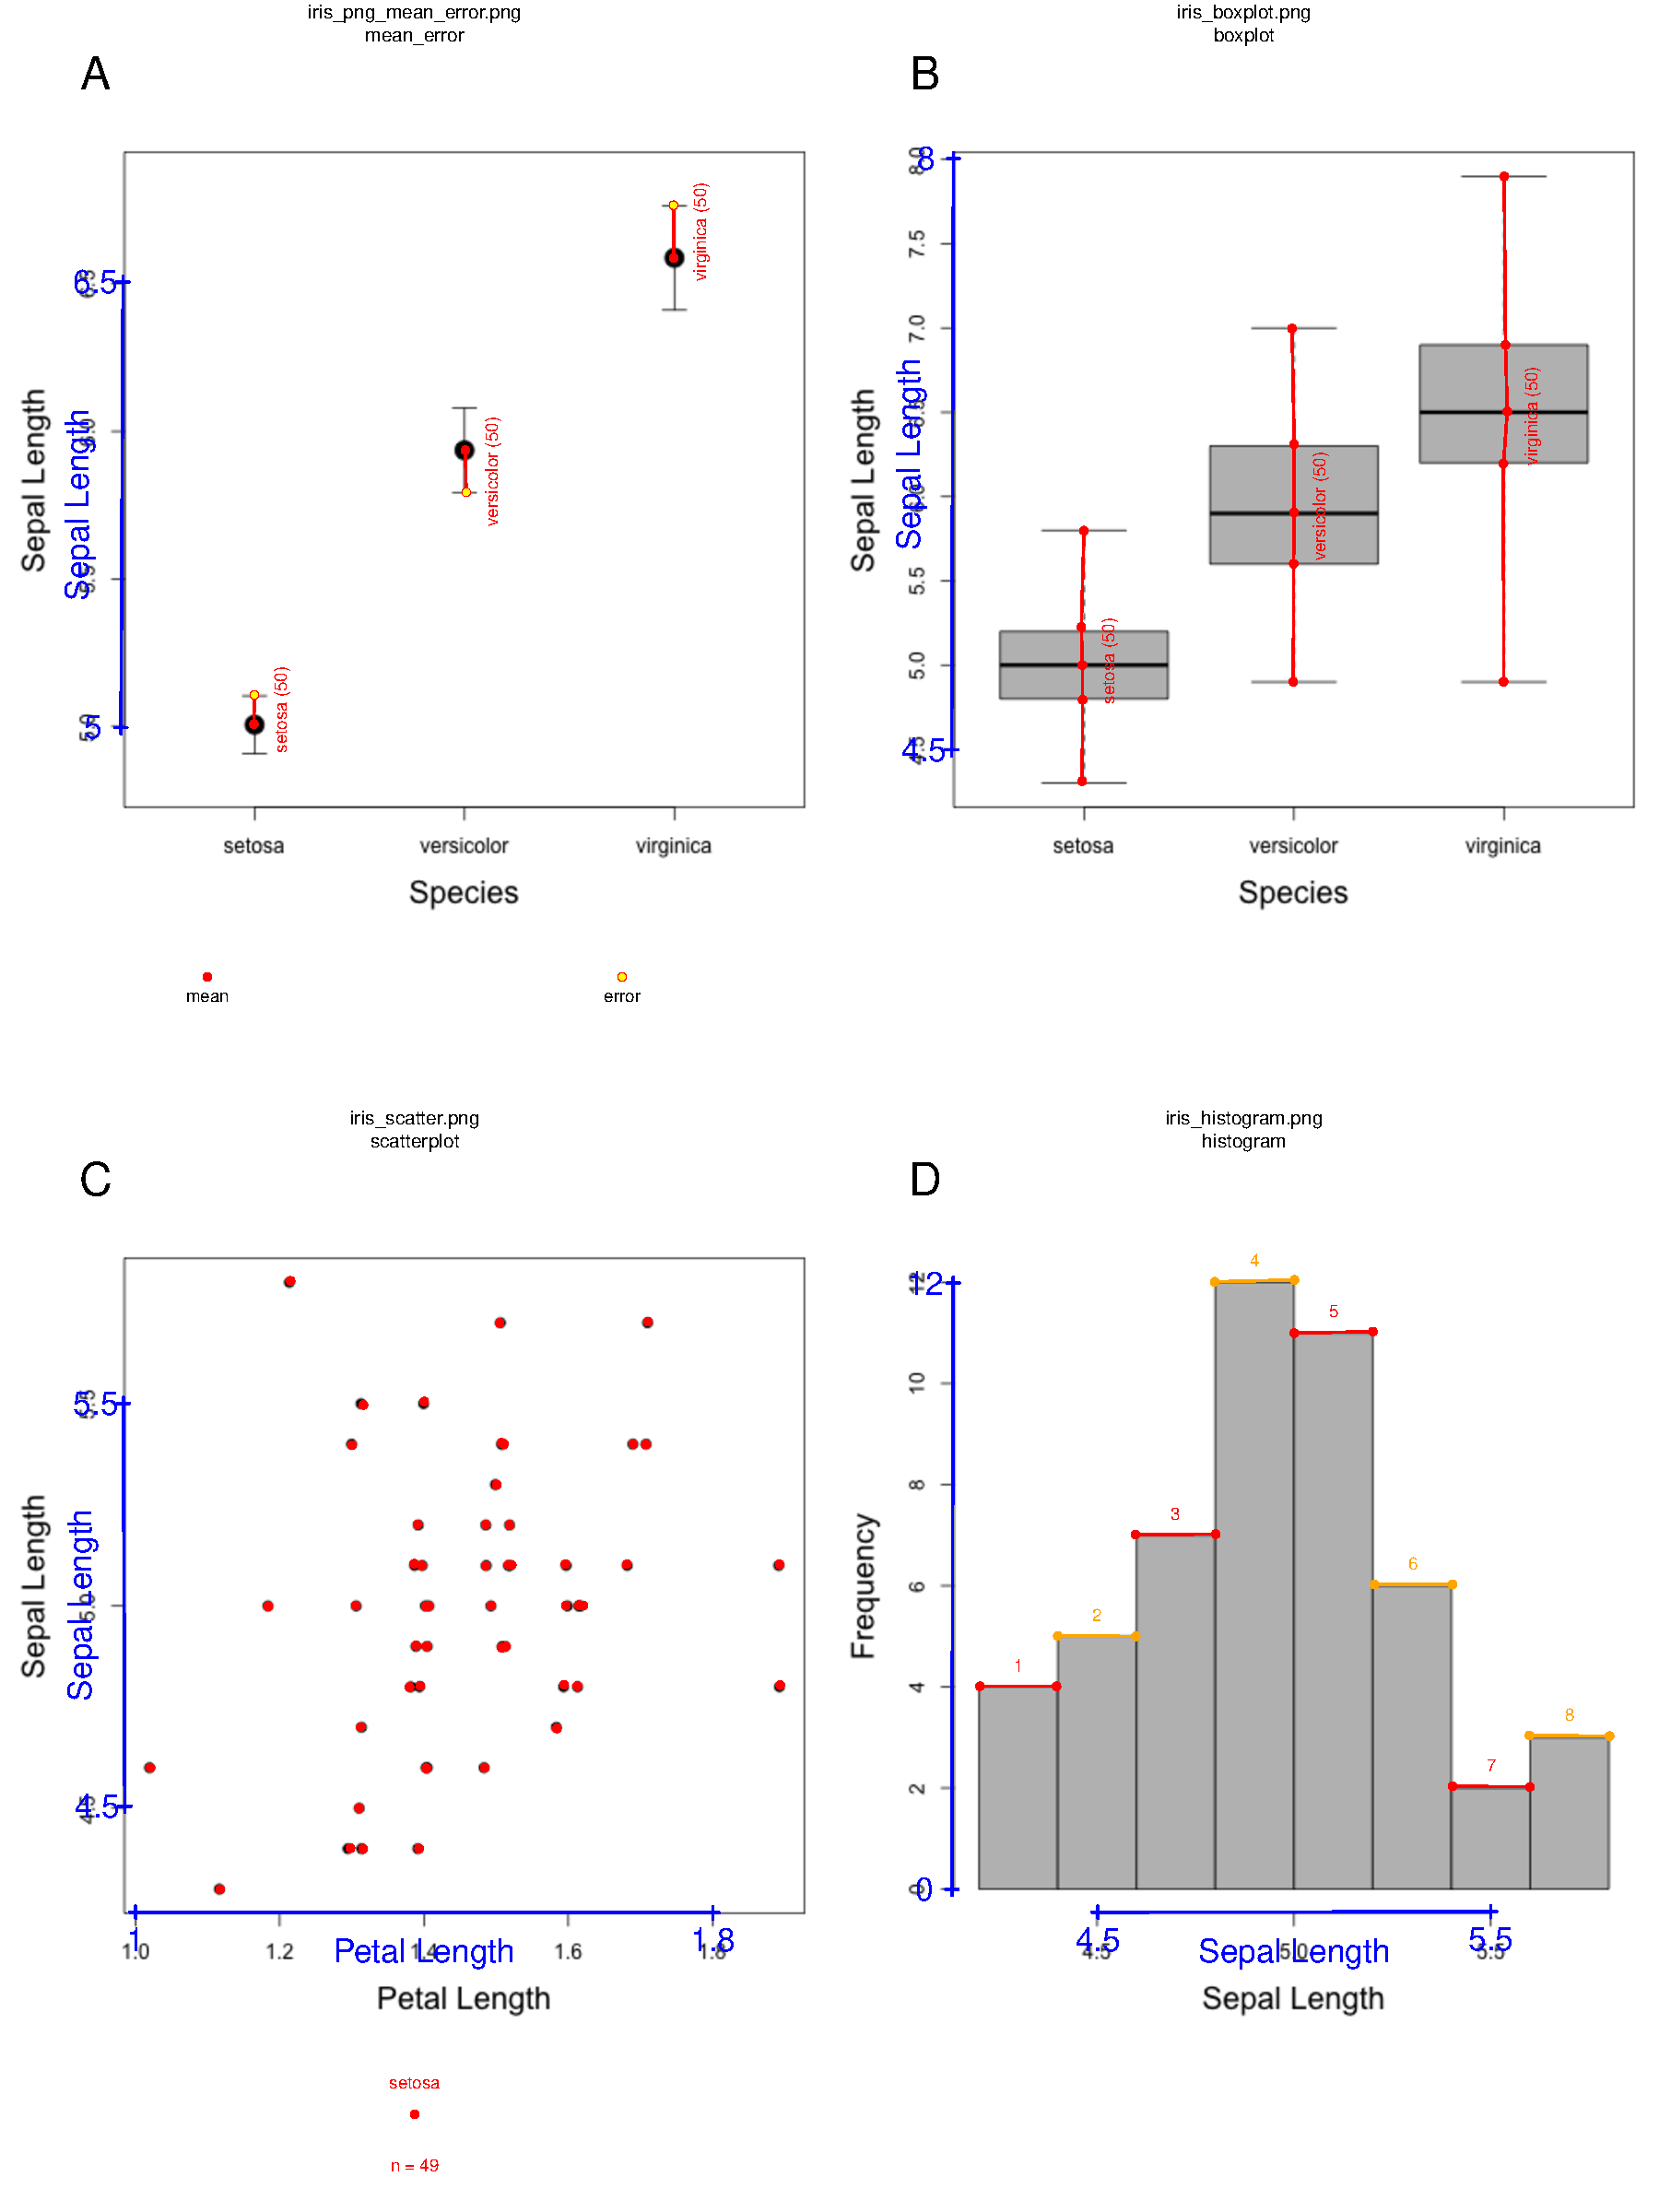
\includegraphics[width=0.75\textwidth]{fig_all_extract.pdf} 
 \caption{Four plot types that \pkg{metaDigitise} is designed to extract data from: A) mean/error plot, B) box plot, C) scatter plot and D) histogram. Data is taken from the iris dataset in R. A and B are plotted with the whole dataset, C and D are just the data for the species \textit{setosa}. Digitisation of the images is shown. All figures are clearly labelled at the top to remind users of the filename and plot type. This reduces errors throughout the digitisation process. Names of the variables and calibration (in blue) are plotted alongside the digitised points. In A) and B), user entered group names and sample sizes are displayed beside the relevant points. In C) the names and sample sizes for each group are shown below the figure.}
\label{fig:all_extract}
\end{figure}


\begin{figure}[!b] 
\centering
 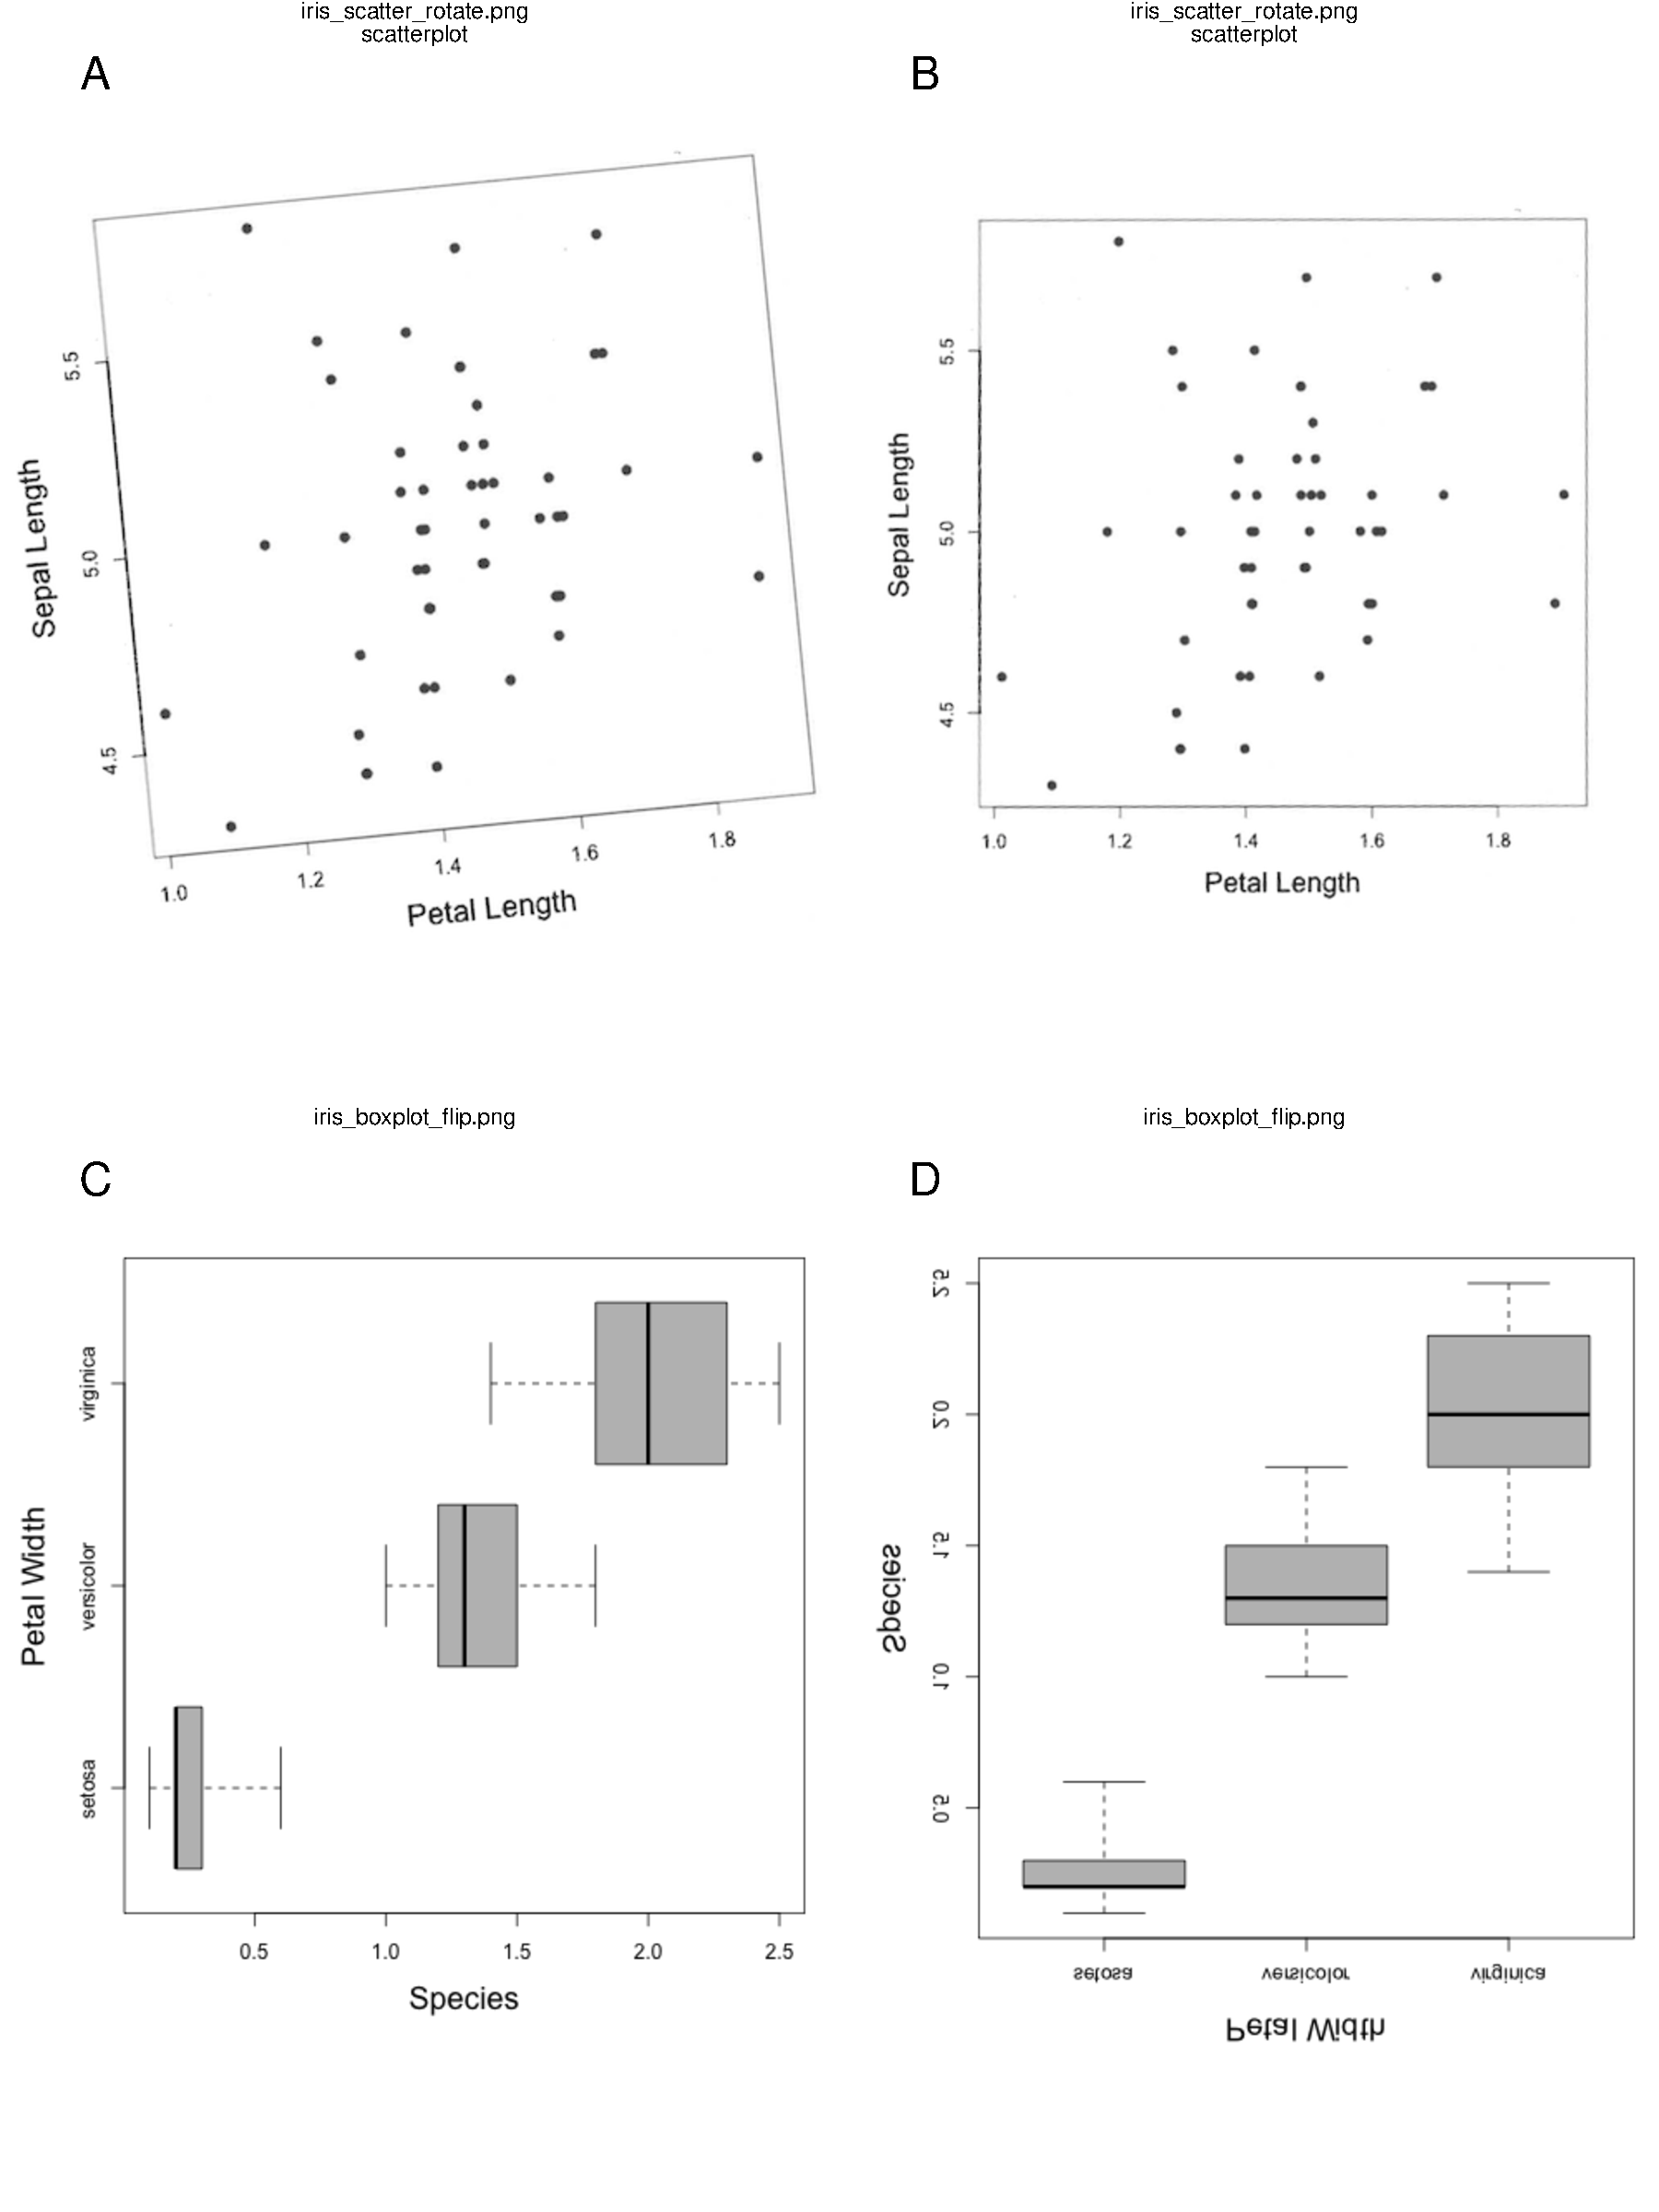
\includegraphics[width=0.75\textwidth]{fig_rotate.pdf} 
 \caption{Figure rotation. A) and B) show how non-aligned images can be realigned through user defined rotation. C) and D) show how figures can be re-orientated so as to aid data input.}
\label{fig:rotate}
\end{figure}



\end{document}
